%(BEGIN_QUESTION)
% Copyright 2010, Tony R. Kuphaldt, released under the Creative Commons Attribution License (v 1.0)
% This means you may do almost anything with this work of mine, so long as you give me proper credit

En koks-\textit{kalcinering}-prosess (der petroleumskoks brennes for å redusere hydrogeninnholdet) bruker en stor beholder for å samle opp koksstøv som dannes rundt transportbåndsystemene med hette. Nivået av koksstøv i beholderen måles med et instrument basert på gammastråling:

$$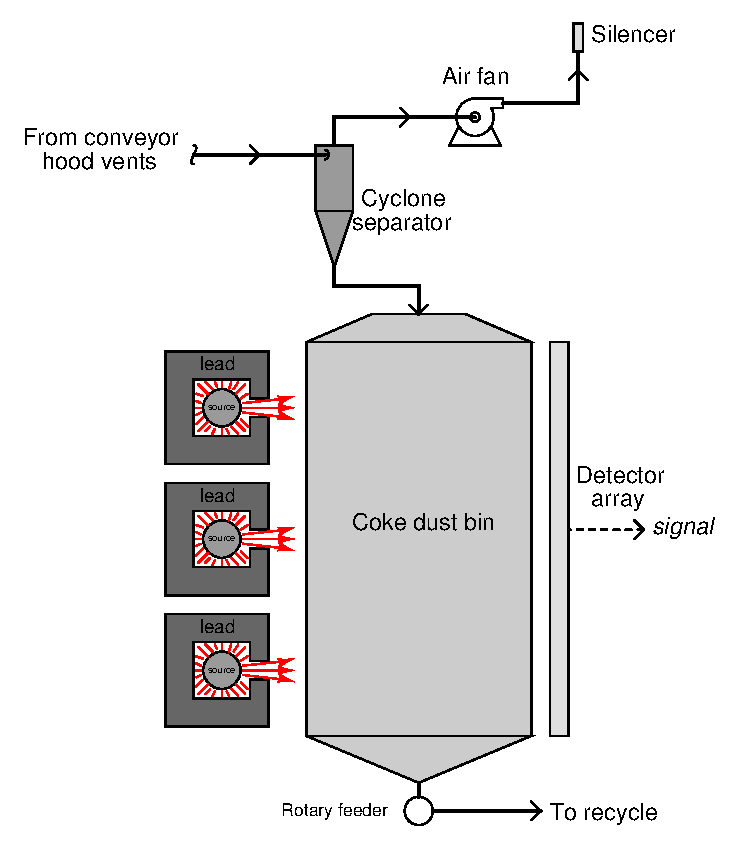
\includegraphics[width=15.5cm]{i00320x01.eps}$$

Forklar hvordan dette systemet bruker kjernefysisk stråling til å måle nivået av koksstøv.

\vskip 20pt \vbox{\hrule \hbox{\strut \vrule{} {\bf Forslag til sokratisk diskusjon} \vrule} \hrule}

\begin{itemize}
\item{} Hvorfor bruker dette systemet flere radioaktive kilder? Hvorfor tror du én kilde ikke er nok?
\item{} Anta at noe radioaktivt materiale ved et uhell havnet i lagringsbeholderen sammen med koksstøvet. Ville dette flytte instrumentets \textit{nullpunkt}, \textit{span}, eller begge deler?
\item{} Nevn noen alternative teknologier vi kunne brukt for å måle nivået av koksstøv.
\item{} Hvilken funksjon har en \textit{syklonseparator}, basert på en analyse av dette enkle prosessflytskjemaet? Merk: syklonseparatorer brukes ofte i sagbruk for å håndtere flis i en luftstrøm.
\end{itemize}

\underbar{file i00320}
%(END_QUESTION)





%(BEGIN_ANSWER)

%(END_ANSWER)





%(BEGIN_NOTES)

Ethvert stoff som plasseres i banen til kjernefysisk stråling, vil dempe strålingen i en viss grad. Dempingen avhenger av strålebanens lengde og materialets tetthet.

\vskip 10pt

Sikkerhetsforhold:

\begin{itemize}
\item{} Hvordan strålingskilden kan ``slås av''
\item{} Sikre at kilden peker riktig vei
\item{} Begrense personells eksponeringstid i strålebanen
\item{} Opprettholde sikre avstander for å utnytte strålingens \textit{invers-kvadrat-lov}
\end{itemize}


%INDEX% Measurement, level: radiation (nuclear)
%INDEX% Process: coke dust storage tank level

%(END_NOTES)
